% !TEX root = ../main.tex

\chapter{绪论}



\section{软件供应链}
随着容器、微服务等新技术日新月异,开源软件成为业界主流形态,软件行业快速发展。现代软件大多数是被“组装”出来的,不是被“开
发”出来的。据 Forrester 统计,软件开发中, 80-90\%的代码来自于开源软件。 因此,现代软件的源代码绝大多数是混源代码,由企业自
主开发的源代码和开源软件代码共同组成。

根据奇安信代码安全实验室的检测与统计\cite{qianxin.com},八个典型的开源软件包生态系统发展迅猛,呈现繁荣态势,包括Maven、NPM、Packagist、Pypi、Godoc、Nuget、Rubygems、Swift。2019年与2020年各开源软件包生态系统增长情况如图\ref{fig:qianxin}:

\begin{figure}[!htp]
  \centering
  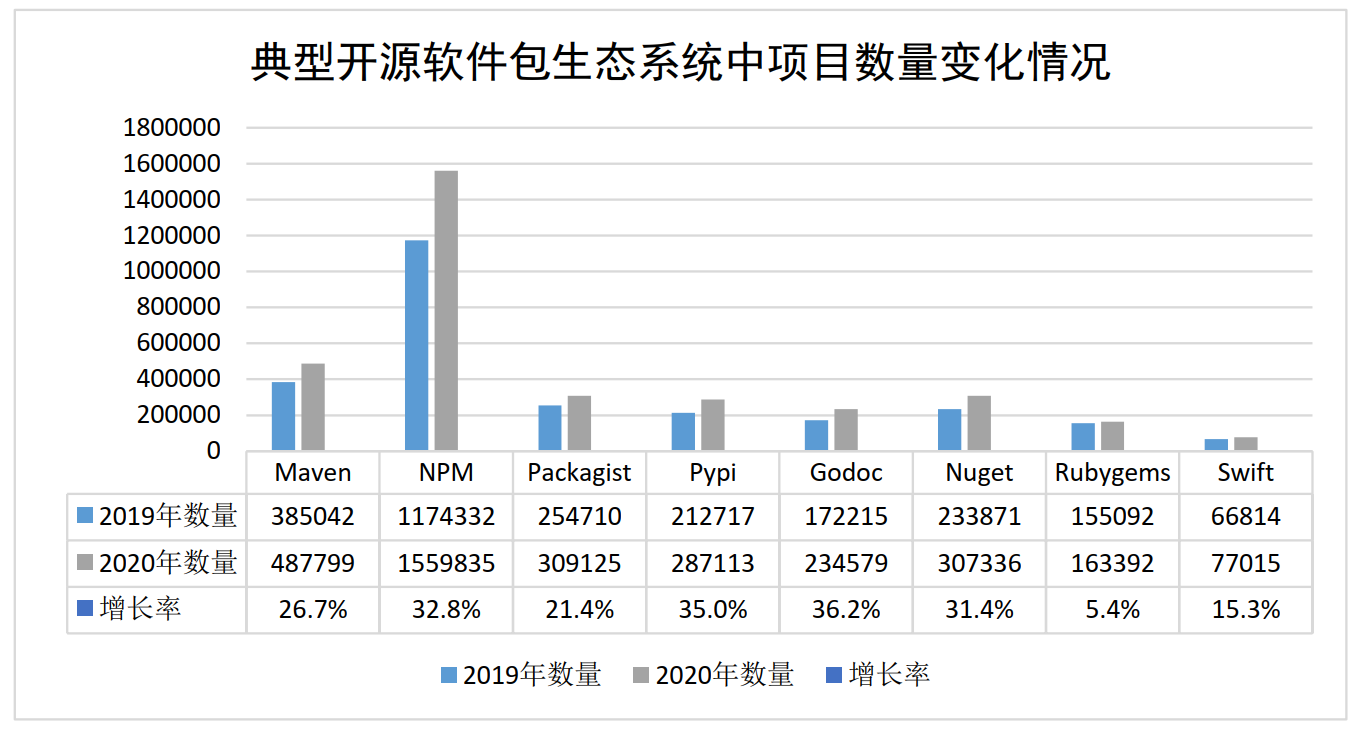
\includegraphics[width=12cm]{qianxin.png} \\
  \caption{2019和2020年八个典型开源软件包生态系统的增长情况}
 \label{fig:qianxin}
\end{figure}

\section{软件供应链安全}
软件供应链的上游软件可能悄无声息地影响着下游产品。开源软件之间的依赖关系错综复杂,在开发过程中,开发者通常借助包管理程序实现自动管理,因此可能意识不到产品中包含里数量巨大的开源软件。一旦某个上游的开源软件被发现安全漏洞,软件开发者无法立即意识到漏洞同时被引入到了产品中,隐含里巨大的软件供应链安全风险。

2020年5月,GitHub披露了Octopus Scanner漏洞\cite{octopus},该漏洞是针对Apache NetBeans IDE项目的开源软件供应链攻击,影响到了26个开源项目。

2020 年 12 月,安全公司FireEye发现全球著名的网络安全管理软件供应商 SolarWinds遭遇国家级 APT 团伙高度复杂的供应链攻击。该攻击在SolarWinds的一个数字签名组件DLL中插入后门,该后门通过HTTP协议与第三方服务器通信。

\section{安卓软件的供应链安全}
Appbrain\cite{appbrain}追踪了450个流行的库,统计结果显示它们在安卓生态系统中有着广泛的使用,广告库、社交网络库、以及手机设备分析库尤为受欢迎。如此广泛的第三方库使用在加速开发过程、避免重复造轮子的同时,也吸引着攻击者将目标向软件供应链上游移动,通过利用受欢迎的库的漏洞来达到攻击应用的目的。atvhunter 2-4。来自Trend Micro的安全研究团队披露百度提供的SDK中的Moplus包含的功能可能被恶意使用,以向用户设备植入后门\cite{baidu}。这一处于软件供应链上游的漏洞已经流入超过14000款安卓APP,可能使得约1亿用户处于黑客的攻击风险中。

2022年4月Google Play商店内的安卓应用超过260万,3月与4月新增应用数量均在2万左右,来自其他市场的应用更是不计其数。

如此数量的APP包含着不可忽视的供应链风险,但是由于APP包含着敏感信息或者具有商业价值的运行逻辑,大部分开发者基于安全和产权的考虑都会将产品进行混淆后再发布。这导致在对APP进行安全性检查时更加困难,识别混淆APP中引入的上游软件成为了亟待解决的问题。事实上,约78\%的漏洞都是在间接的依赖中找到,可能带来的安全风险则更加难以发现\cite{qianxin.com}。






\chapter{研究现状}

\section{检测混淆库}
随着APP混淆技术的成熟,以第三方库能够被容易地区分为前提的方法已不适用,标识符被混淆为无意义的简短的字母组合,比如\textit{com.google}可能被混淆为\textit{a.c},无法提供关于库的任何信息。图\ref{fig:hunxiao}为一个代码混淆的示例,仅从名称无法获得任何关于包的信息。

\begin{figure}[!htp]
  \centering
  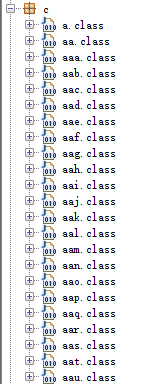
\includegraphics[width=3cm]{hunxiao.png} \\
  \caption{一款360软件的apk解压后得到的经过重命名混淆的class文件}
 \label{fig:hunxiao}
\end{figure}

T. Book等人的工作通过白名单的方法检测APP内的第三方库\cite{book2013longitudinal},但这类方法显然无法解决标识符重命名的问题。PEDAL\cite{liu2015efficient}借助机器学习方法,从SDK中提取代码特征,并使用包之间的关系信息训练了分类器来识别第三方库。


\section{检测未知库}

一些研究工作提出了在没有已知第三方代码的数据库知识情况下检测APP组成成分的方法。此类方法通常首先把开发者代码与第三方代码进行分类,再将第三方代码聚类成不同的组件,组件即一个可能的库的候选,进一步评估候选之间的相似度,当超过相似度阈值的候选的出现次数足够多时就认为找到了一个库。

如Chen等人\cite{chen2016following}从大量的APP中获取库,进行聚类和检测然而这一方法在混淆的情况下表现不佳,因为其假设不同APP中包含的库的相同实例拥有相同的包名,混淆打破了这一基本的假设。

为解决包名混淆问题,LibRadar\cite{ma2016libradar}使用特征哈希的方法,不需要基于包名的聚类,而是借助包中的目录结构来识别库的候选,具体来说是将一个候选表示为一个目录树的结构。这引入一个新的假设,即包的结构在混淆过程中不改变。但混淆工具可以将不同的包合并为一个包,很容易打破这一假设。

WuKong\cite{wang2015wukong}和AnDarwin\cite{crussell2014andarwin}用控制流图和API数量来定义哈希特征,用来计算各候选库的相似度。考虑到混淆工具可能修改一个方法的控制流图,或者移除在APP运行中未真正使用的方法,哈希的质量影响着这两类方法的表现性能。


\section{检测已知库}

基于已知库的检测要求关于现存库的知识,如库的基本信息、哈希特征等,在混淆APP第三方库识别的场景下,用构建知识数据库的代价换取了更好的表现。

具有代表性的一个工具是LibScout\cite{backes2016reliable},用包的结构以及类的哈希作为特征,进行APP与数据库中第三方库的匹配,在控制流篡改和包/类/描述符重命名情况下依然有效。但是随着数据库中的标准库代码特征增多,哈希特征的计算也应当考虑更多信息,导致特征生成时间与匹配时间增加。



\section{检测标准库的版本}

现有工作中以版本为目标实现精确检测的并不多,AdDetect\cite{narayanan2014addetect}仅能够区分广告和非广告的库,基于聚类的方法如LibRadar\cite{ma2016libradar},LibD\cite{li2017libd}等都没有声明能够检测库的特定版本。

实现版本的检测仍面临着很多问题:
\begin{enumerate}
\item{需要处理庞大的数据集。第三方库本身就纷繁复杂,如果再将各个版本考虑进去,将导致需要处理的数据成倍增长。}
\item{缺乏精确的表示。一个库的不同版本可能差异微小,如何找到合适的特征来区分这一差别非常关键。}
\item{代码混淆的干扰。代码混淆同样会导致库的代码发生改变,这种改变是由不同库引起还是由同一库的不同版本引起,需要被准确的区分。}
\end{enumerate}



\chapter{研究方法}

在参考了多篇文献后,我提出了一种适用于包的结构混淆、包/类/标识符重命名场景的,基于已知标准库的数据库,利用两类信息生成粗粒度/细粒度两级哈希特征的安卓应用第三方库及其特定版本的检测方法。



\section{方法概述}

此方法不依赖于包中的目录结构以及各级名称,因此可以抵抗结构混淆以及重命名混淆,包括了四个步骤:
\begin{enumerate}
\item{预处理jar、aar和apk。将来自Maven仓库的jar包、aar包以及待检测apk处理成便于构建树结构的形式。}
\item{构建特征树。根据上一阶段输出,将每个包作为根节点构建特征树,该包内的所有类,不论是根包的类还是子包的类,一律作为树的中间层节点,各类的方法作为叶子节点。特征分为粗粒度、细粒度两级特征。粗粒度特征为方法的描述符的返回值以及参数类型,细粒度特征为该方法的字节码,首先生成叶子节点的两级特征,再利用叶子节点生成中间层节点即类节点的特征。}
\item{构建数据库与匹配。根据以上特征生成方法,计算Maven仓库中的标准库的特征,并存储到数据库中。对待检测APP,首先生成粗粒度特征,确定所包含的库,再根据细粒度特征,确定各库的具体版本。}
\end{enumerate}



\section{包的预处理}

\subsection{Dex与Class文件的处理}

\subsubsection{Dex与Class简介}

\textbf{DEX文件:}DEX文件时Android系统中的一种文件,是一种特殊的数据格式,能够被Dalvik虚拟机识别并加载执行,类似于Windows上的EXE可执行文件。将APK安装包解压后得到的文件就包含了DEX文件,它记载了应用程序的全部操作指令以及运行时数据。当java程序编译成class文件后,还需要使用dx工具将所有的class文件整合到一个DEX文件里,目的是其中各个类能够共享数据,在一定程度上降低了冗余,同时也使文件结构更加紧凑。DEX文件大小通常是传统jar包的50\%左右。


\textbf{CLASS文件:}class文件是能够被java虚拟机识别,加载并执行的文件格式,通过javac程序可以从java源文件生成class文件。class文件记录了一个类文件的所有信息,不仅包含了java源代码中的信息,还包括了this、super等关键字的信息。作为一种8位字节的二进制六文件,class中的数据按顺序紧密排列,没有间隙,从而让JVM加载更加迅速,每一个类、接口或者枚举都单独占据一个class文件。


\subsubsection{Dex与Class获取}








